
\documentclass{article}

% Deactivate sectsty warning when loading sectsty {{{
\usepackage[immediate]{silence}
\WarningFilter[temp]{latex}{Command}
\usepackage{sectsty}
    \sectionfont{\normalfont\sffamily\bfseries\color{blue!40!black}}
    \subsectionfont{\normalfont\sffamily\bfseries\color{blue!30!black}}
\DeactivateWarningFilters[temp]
\makeatletter % disable the runtime redefinitions
\let\SS@makeulinesect\relax
\let\SS@makeulinepartchap\relax
\makeatother
% }}}

\usepackage[margin=4cm]{geometry}
    \setlength\parindent{0pt}
\usepackage{fancyhdr}
    \pagestyle{fancy}
\usepackage{fontspec}
    \setsansfont{Linux Biolinum O}
\usepackage{polyglossia}
    \setmainlanguage{english}
\usepackage{sectsty}
    \sectionfont{\normalfont\sffamily\bfseries\color{blue!40!black}}
    \subsectionfont{\normalfont\sffamily\bfseries\color{blue!30!black}}
\usepackage{amsmath}
\usepackage{amssymb}
\usepackage{siunitx}
\usepackage{float}
\usepackage{booktabs}
\usepackage{subcaption}
\usepackage{graphicx}
\usepackage{xcolor}
\usepackage{pdfpages}
\usepackage{listings}
    \lstset{language=c++,
	basicstyle=\tiny\ttfamily,
	breaklines=true,
	framextopmargin=50pt,
	frame=bottomline,
	backgroundcolor=\color{white!86!black},
	commentstyle=\color{blue},
	keywordstyle=\color{red},
	stringstyle=\color{orange!80!black}}
\usepackage{tikz}

\title{\textsf{\color{blue!40!black}Übungsblatt 1}}
\author{Maurice Donner \and Jan Hubrich \and Adrian Müller}

\begin{document}

\maketitle

\includepdf[pages=-]{Aufgabe_1.pdf}
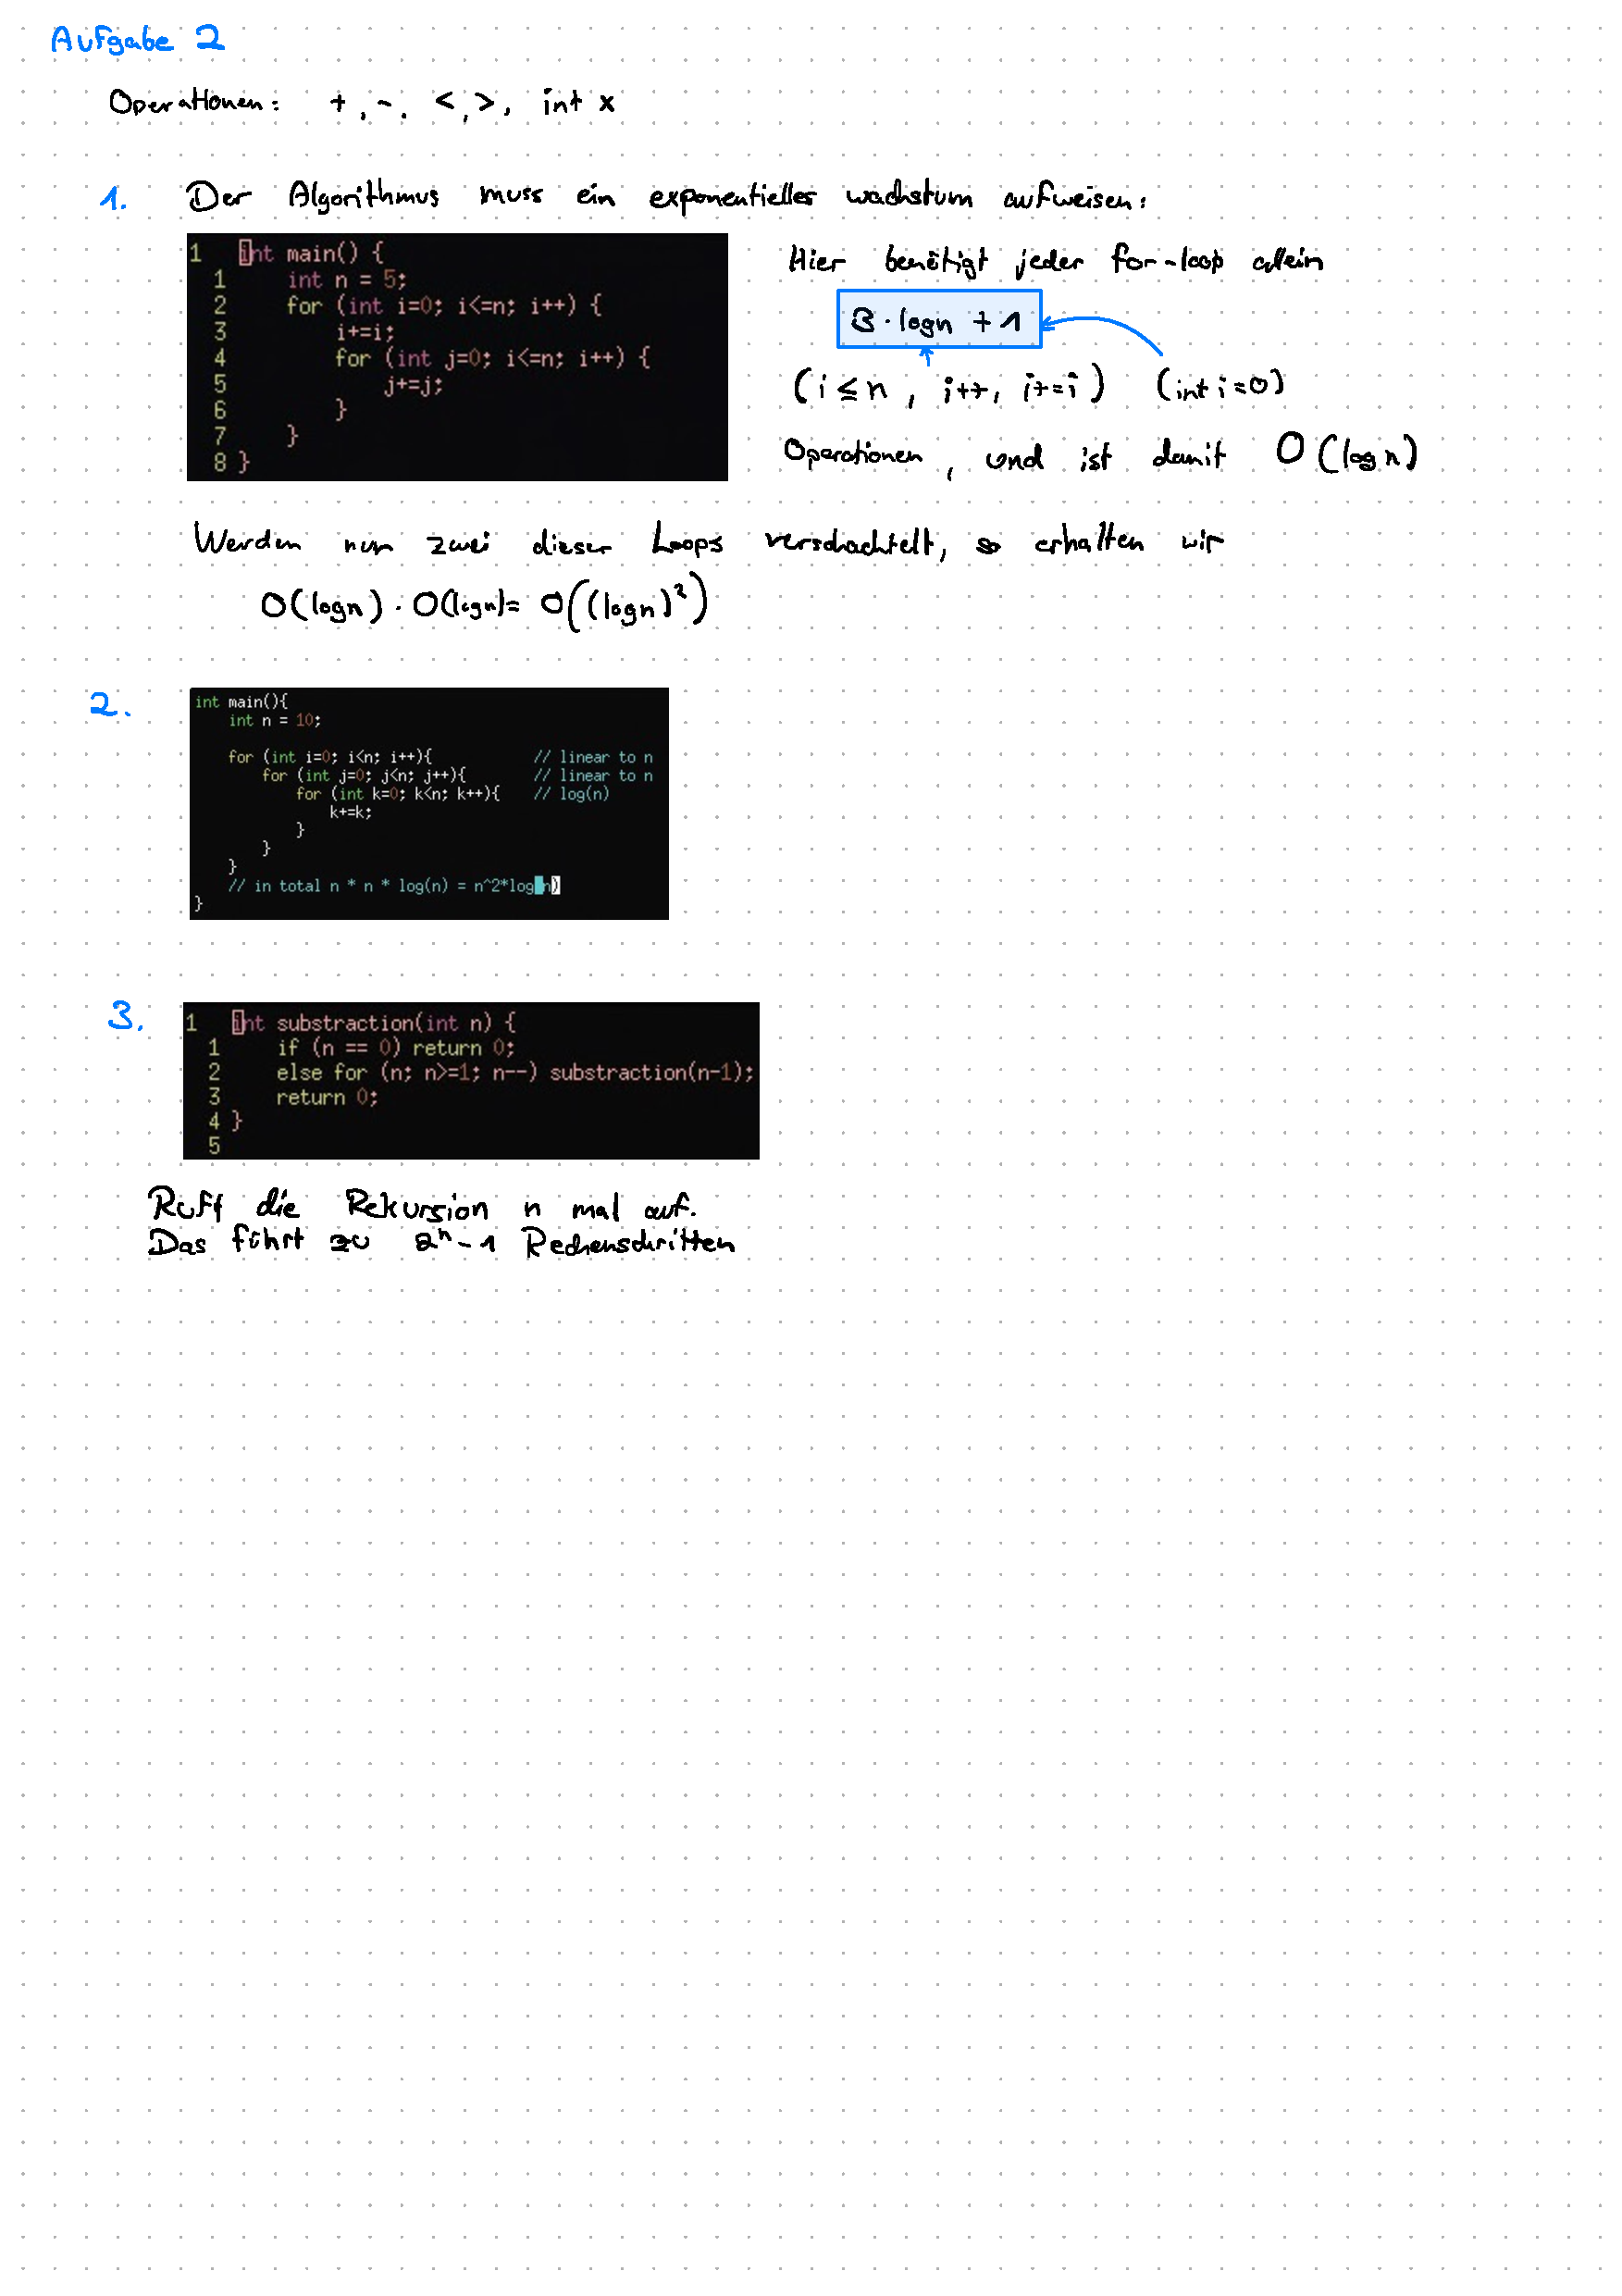
\includepdf{Aufgabe_2.pdf}
\section*{Aufgabe 3}
The code can be found in the file \texttt{Aufgabe\_3.cpp}. The code is commented,
so every step can be followed. The program \texttt{Aufgabe\_3} can be run
and takes a string of zeros and ones as console input, followed by the
variable bitlength \texttt{k}.\\
The algorithm is of the order \( \mathcal{O}(n) \), because it's based
on the recursive divide \& conquer algorithm, where \( d < b \).

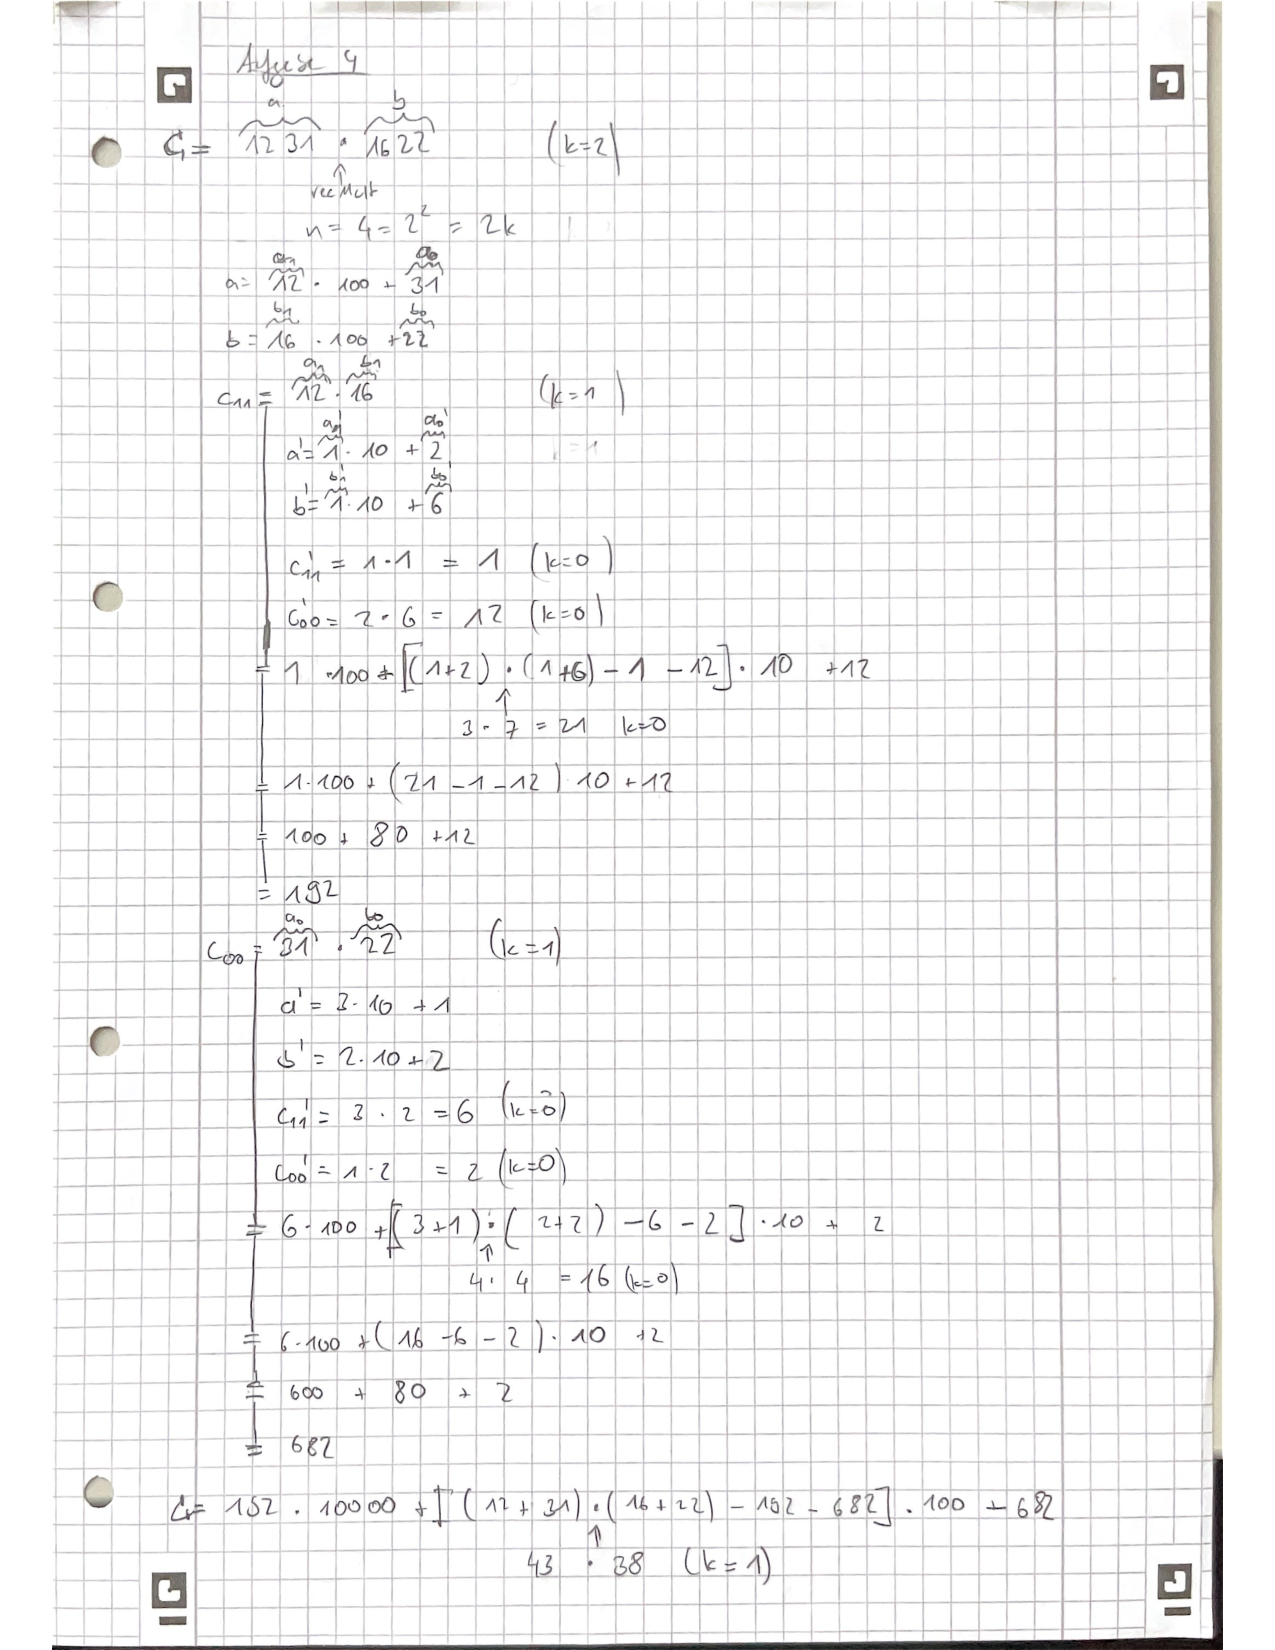
\includepdf[pages=-]{Aufgabe_4.pdf}

\section*{Additional contents}
The code for exercise 3 can be found below

\begin{lstlisting}
#include <iostream>
#include <vector>
#include <string>
#include <bitset>
#include <cmath>

using namespace std;

// converts string of '0' and '1' into an integer
int strtoint(string s){
    int output = 0;

    int count = 0;
    for (int i=s.length()-1; i>=0; --i){
	if (s.at(i) == '1') output += pow(2, count);
	count++;
    }
    return output;
}


int search(string s, int k){// s is the input string containing only '0' and '1's 
			    // k is the bit length of the numbers in s

    int numOfNums = s.length() / k; // calculates the amount of numbers in "s"
    if (numOfNums == 1){    // break condition if divide and conquer has divided and conquered
			    // only one number in bit form is left in string

	if (s.at(k-1) == '1'){ // looks a smallest bit. If it's 1 -> number is uneven, else number is even
	    return strtoint(s) - 1; // -1, because missing number is one less compared to the remaining one
	}
	else{
	    return strtoint(s) + 1; // +1, because missing number is one more compared to the remaining one
	}
    }

    int middle_bit = (numOfNums / 2 + 1) * k - 1;   // calculates the index of the smallest bit of the number
						    // in the middle of the array. There is always a "middle number"
						    // because the array has 2^k - 1 numbers in it

    if (s.at(middle_bit) == '1'){   // if the number in the middle is uneven
				    // the missing number has to be to the right,
				    // thus the search interval can be split in 
				    // half (divided). The first half of the
				    // string can be discarded
				    
	s.erase(0, (numOfNums/2+1)*k);		    // divide step
	return search(s, k);			    // recursion step
    }    
    if (s.at(middle_bit) == '0'){   // if the number in the middle is even, the
				    // missing number has to be to the left.
				    // Thus, the last half of the string can 
				    // be discarded.

	s.erase(middle_bit-k+1, (numOfNums/2+1)*k); // divide step
	return search(s, k);			    // recursion step
    }   
    // after one iteration the string has 2^(k-1) numbers in it
    // after k-1 iterations, the array is conquered and the break condition
    // is true
}


int main(){
    string s;
    int k = 2;
    cout << "Please input the string" << endl;
    cin >> s;
    cout << "Please input the bitlength k" << endl;
    cin >> k;

    int lostNum = search(s, k);
    
    cout << "The lost Number is: "  << lostNum << endl;

    return 0;
}
\end{lstlisting}


\end{document}

